\section{Reference}
\label{reference_csp}

\subsection{Observers}
\label{observers_csp}

\subsubsection{Formula Observer}

The formula observer observes a list of formulas (i.e. expressions) and triggers a function whenever a state change occurred.
The result of the formulas are passed to the trigger function.
The following options can be passed:

\begin{tabular}{ l l l p{7cm} }
  \textbf{Name} & \textbf{Type} & \textbf{Default} & \textbf{Description} \\
  \hline\noalign{\medskip}
  formulas & list / function* & empty list & Define a list of expressions that should be evaluated and passed to the trigger function.\\
  \hline\noalign{\medskip}
  cause & string / function* & '\textit{AnimationChanged}' & The trigger cause. Possible values: '\textit{AnimationChanged}', '\textit{ModelChanged}' and '\textit{ModelInitialised}'. \\
  \hline\noalign{\medskip}
  trigger & function &  & The trigger function will be called after every state change with its \textit{origin} reference set to the element that the observer is attached to and the requested \textit{data} (the result of the expressions). \\
\end{tabular}

*This attribute also accepts a function that should return its value.

\begin{lstlisting}[language=JavaScript]
$("#vis").observe("formula", {
  formulas: ["N"],
  trigger: function (origin, data) {
    origin.text(data.values[0].value);
  }
})
\end{lstlisting}

\subsubsection{CSP Event Observer}

The mathematical semantics of CSP are mainly based on \textit{traces}.
A trace is a sequence of events performed by a process that can communicate and interact with other processes within the CSP model.
The basic idea of the CSP visualisation approach is to visualise the information encoded in the given sequence of events (\textit{trace}).
However, a process may perform many different traces and thus creating a visualisation manually for each possible trace is an almost impossible task.

The presented approach requires the user to set up only one visualisation that may be capable of representing any possible trace of a CSP process of a particular model. 
This is achieved by means of \textit{observers}) that are used to link the visualisation with the model.

We extended BMotion Studio with a new observer type called \textit{CSP event observer} in order to support creating visualisations of CSP models.
The observer has the following structure:

\begin{lstlisting}[language=JavaScript]
{ "exp": "<user-defined CSP expression>", 
  "actions": [ 
    { "selector":"<selector>", "attr":"<attribute>", "value":"<value>" },
    { ... }
  ] }
\end{lstlisting}

Each observer has a \textit{user-defined CSP expression} and a list of \textit{actions}.
The user-defined expression constitutes a set of observed events, whereas the actions determine the changes made on visual elements.

An action defines a \textit{selector} that matches a set of visual elements in the visualisation (SVG graphic). 
A selector follows the syntax provided by jQuery\footnote{For more information about jQuery and selectors we refer the reader to the jQuery API documentation \url{http://api.jquery.com/category/selectors/}.}. 
For instance, to match the visual element with the ID ``elem1'' (each element should have a unique ID in the visualisation) the user can define the selector ``\#elem1''. 
The prefix ``\#'' is used for matching a visual element by its ID in jQuery. 
An action also defines an \textit{attribute} (e.g. ``fill'' for colouring the interior of a visual element like a circle shape) and a corresponding \textit{value} that will be set as the new value of the attribute when the action is triggered.
The actions of an observer $o$ are triggered when the currently processed event is in the set of observed events of $o$.

The user can refer to the information given by the arguments of the currently processed event within the action fields (selector, attribute and value).
This is achieved by means of the construct ``\{\{aN\}\}'' where aN refers to the N-th argument of the event.
For instance, if the event has two arguments, then the first and the second one can be obtained with ``\{\{a1\}\}'' and ``\{\{a2\}\}'', respectively. 
To illustrate this, consider an event $evt.x$ with $x \leftarrow 0..4$.
One may want to use the information given by the first argument $x$ of $evt$ within a selector in order to match visual elements that have an ID of the form ``elem$x$''.
This can be done by defining the selector ``\#elem\{\{a1\}\}''.
The construct ``\{\{a1\}\}'' will be replaced by the value of the first argument of the currently processed event in the observer.
For instance, if the currently processed event is $evt.2$, the selector ``\#elem\{\{a1\}\}'' will become ``\#elem2''.

\begin{figure}[h!]\centering
	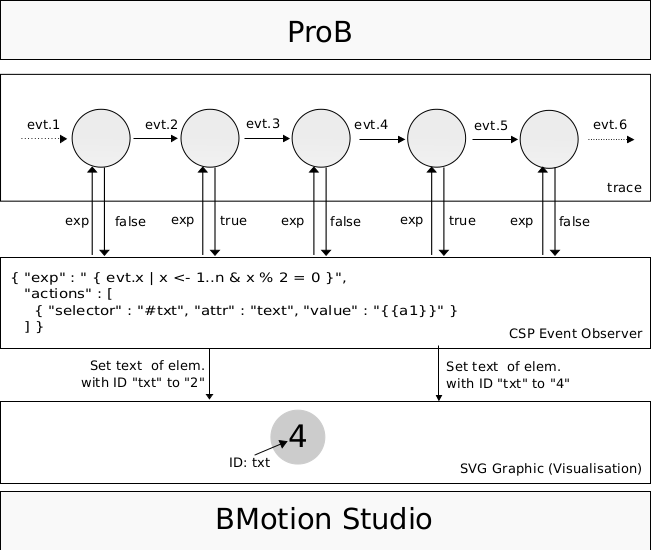
\includegraphics[width=14cm]{img/reference/detailprocess}
	\caption{The function of the CSP event observer}
	\label{fig:detailprocess}
\end{figure}

Fig.~\ref{fig:detailprocess} illustrates the function of the CSP event observer on a simple example.
The visualisation consists of an SVG graphic with a text field element with the ID ``txt'' and one CSP event observer.
The CSP event observer defines an expression that constitutes the set of observed events $evt = \{evt.2, evt.4, evt.6, ..\}$ and one action $act1$ that changes the value of the attribute "text" to ``\{\{a1\}\}'' of the visual element with the ID ``txt'' (the text field).
The observer is executed for each event of a given trace.
This means that, whenever the currently processed event is in the set of observed events $evt$, the observer will trigger the defined action $act1$.
For instance, the execution of the event $evt.4$ causes the observer to set the value of the text field element to ``4'' as demonstrated in Fig.~\ref{fig:detailprocess}.

In general the observer is attached to a parent visual element.
The actions of the observer are applied on the children.
The following options can be passed:

\vspace{0.5cm}
\begin{tabular}{ l l l p{7cm} }
  \textbf{Name} & \textbf{Type} & \textbf{Default} & \textbf{Description} \\
  \hline\noalign{\medskip}
  selector & string / function* & & The selector that matches the parent visual element. \\
  \hline\noalign{\medskip}
  cause & string / function* & '\textit{AnimationChanged}' & The trigger cause. Possible values: '\textit{AnimationChanged}', '\textit{ModelChanged}' and '\textit{ModelInitialised}'. \\  
  \hline\noalign{\medskip}
  observers & list & empty list & Define a list of CSP event observers. \\
  \hline\noalign{\medskip}
  : exp & string / function* & & The user-defined expression that constitutes a set of observed events.\\
  \hline\noalign{\medskip}
  : actions & list & & A list of actions that should be applied on the visual elements. \\
  \hline\noalign{\medskip}
  :: selector & string / function* & & The \textit{selector} matches a set of visual elements. \\
  \hline\noalign{\medskip}
  :: attr & string / function* & & The attribute that should be modified. \\
  \hline\noalign{\medskip}
  :: value & string / function* & & The value that should be set on the attribute. \\
\end{tabular}

*This attribute also accepts a function that should return its value.

\begin{lstlisting}[language=JavaScript]
$("#crossing").observe("csp-event", {
  observers: [
    { exp: "{gate.down,gate.up}",
      actions: [
        {selector: "g[id^=gate]", 
        attr: "opacity", 
        value: "0"}
      ]
    },
    { exp: "{gate.down}",
      actions: [
        {selector: "#gate-go_down-2, #gate-go_down-1", 
         attr: "opacity", 
         value: "100"}
      ]
    },
    { exp: "{gate.up}",
      actions: [
        {selector: "#gate-go_up-2, #gate-go_up-1", 
        attr: "opacity", 
        value: "100"}
      ]
    },
    { exp: "{enter.x.y | x <- {0..4}, y <- {Train1,Train2}}",
      actions: [
        {selector: "#train_{{a2}}", 
        attr: "x", 
        value: "{{a1}}00"},        
        {selector: "#train_{{a2}}", 
        attr: "transform", 
        value: ""}
      ]
    },
    { exp: "{leave.x.y | x <- {0..3}, y <- {Train1,Train2}}",
      actions: [
        {selector: "#train_{{a2}}", 
        attr: "transform",
        value: "translate(50,0)"}
      ]
    }
  ]
});
\end{lstlisting}